% Options for packages loaded elsewhere
\PassOptionsToPackage{unicode}{hyperref}
\PassOptionsToPackage{hyphens}{url}
%
% DOCUMENT CLASS
% =============================================
\documentclass[openleft,10pt]{article}
\usepackage{lmodern}
\usepackage{amssymb,amsmath}
\usepackage{ifxetex,ifluatex}
\ifnum 0\ifxetex 1\fi\ifluatex 1\fi=0 % if pdftex
  \usepackage[T1]{fontenc}
  \usepackage[utf8]{inputenc}
  \usepackage{textcomp} % provide euro and other symbols
\else % if luatex or xetex
  \usepackage{unicode-math}
  \defaultfontfeatures{Scale=MatchLowercase}
  \defaultfontfeatures[\rmfamily]{Ligatures=TeX,Scale=1}
\fi
% Use upquote if available, for straight quotes in verbatim environments
\IfFileExists{upquote.sty}{\usepackage{upquote}}{}
\IfFileExists{microtype.sty}{% use microtype if available
  \usepackage[]{microtype}
  \UseMicrotypeSet[protrusion]{basicmath} % disable protrusion for tt fonts
}{}
\makeatletter
\@ifundefined{KOMAClassName}{% if non-KOMA class
  \IfFileExists{parskip.sty}{%
    \usepackage{parskip}
  }{% else
    \setlength{\parindent}{0pt}
    \setlength{\parskip}{6pt plus 2pt minus 1pt}}
}{% if KOMA class
  \KOMAoptions{parskip=half}}
\makeatother
\usepackage{xcolor}
\IfFileExists{xurl.sty}{\usepackage{xurl}}{} % add URL line breaks if available
\IfFileExists{bookmark.sty}{\usepackage{bookmark}}{\usepackage{hyperref}}
\hypersetup{
  hidelinks,
  pdfcreator={LaTeX via pandoc}}
\urlstyle{same} % disable monospaced font for URLs
\setlength{\emergencystretch}{3em} % prevent overfull lines
\providecommand{\tightlist}{%
  \setlength{\itemsep}{0pt}\setlength{\parskip}{0pt}}
\setcounter{secnumdepth}{-\maxdimen} % remove section numbering

\usepackage{fontspec}
  \setmainfont[Ligatures=TeX]{Charter}
  \setsansfont{Lucida Grande}
  \setmonofont{American Typewriter}
  \newfontfamily\chapfont{Charter Black}
  \newfontfamily\secfont{Charter Black}
  \newfontfamily\handfont{Bradley Hand}

\setlength{\paperwidth}{14.194in}
\setlength{\paperheight}{9.861in}
\pdfpagewidth=\paperwidth
\pdfpageheight=\paperheight

\setlength{\textwidth}{14.194in}
\setlength{\textheight}{9.861in}
\setlength{\oddsidemargin}{-1in}
\setlength{\evensidemargin}{-1in}
\setlength{\topmargin}{0in}


\renewcommand{\baselinestretch}{1.1}
\renewcommand{\arraystretch}{1.2}
\setlength{\tabcolsep}{2pt}

\usepackage{fancyhdr}
\pagestyle{fancy}
\fancyhf{} % clear all header and footer fields
\renewcommand{\headrulewidth}{0pt} % remove the header rule
\fancyfoot[C]{\small\thepage} % small page number in the center of the footer
\setlength{\footskip}{36pt}

\usepackage{tikz}
\usepackage{xcolor}
\definecolor{avocadogreen}{rgb}{0.34, 0.51, 0.01} % An example of avocado green
\definecolor{vintageorange}{rgb}{0.95, 0.65, 0.0} % An example of vintage orange
\definecolor{darkavocadogreen}{rgb}{0.20, 0.30, 0.01} % A darker shade of avocado green
\definecolor{darkvintageorange}{rgb}{0.70, 0.40, 0.0} % A darker shade of vintage orange

\pagestyle{empty}\pagecolor{avocadogreen}\color{white}
\begin{document}
\noindent%
\begin{minipage}[t][9.861in][t]{6.625in}
  \noindent
  \centering
  \mbox{ } \hfill
  \hspace{0.5in}
  \begin{minipage}{4.5in}
    % \hspace*{1in}
    % \mbox{ } \hfill
    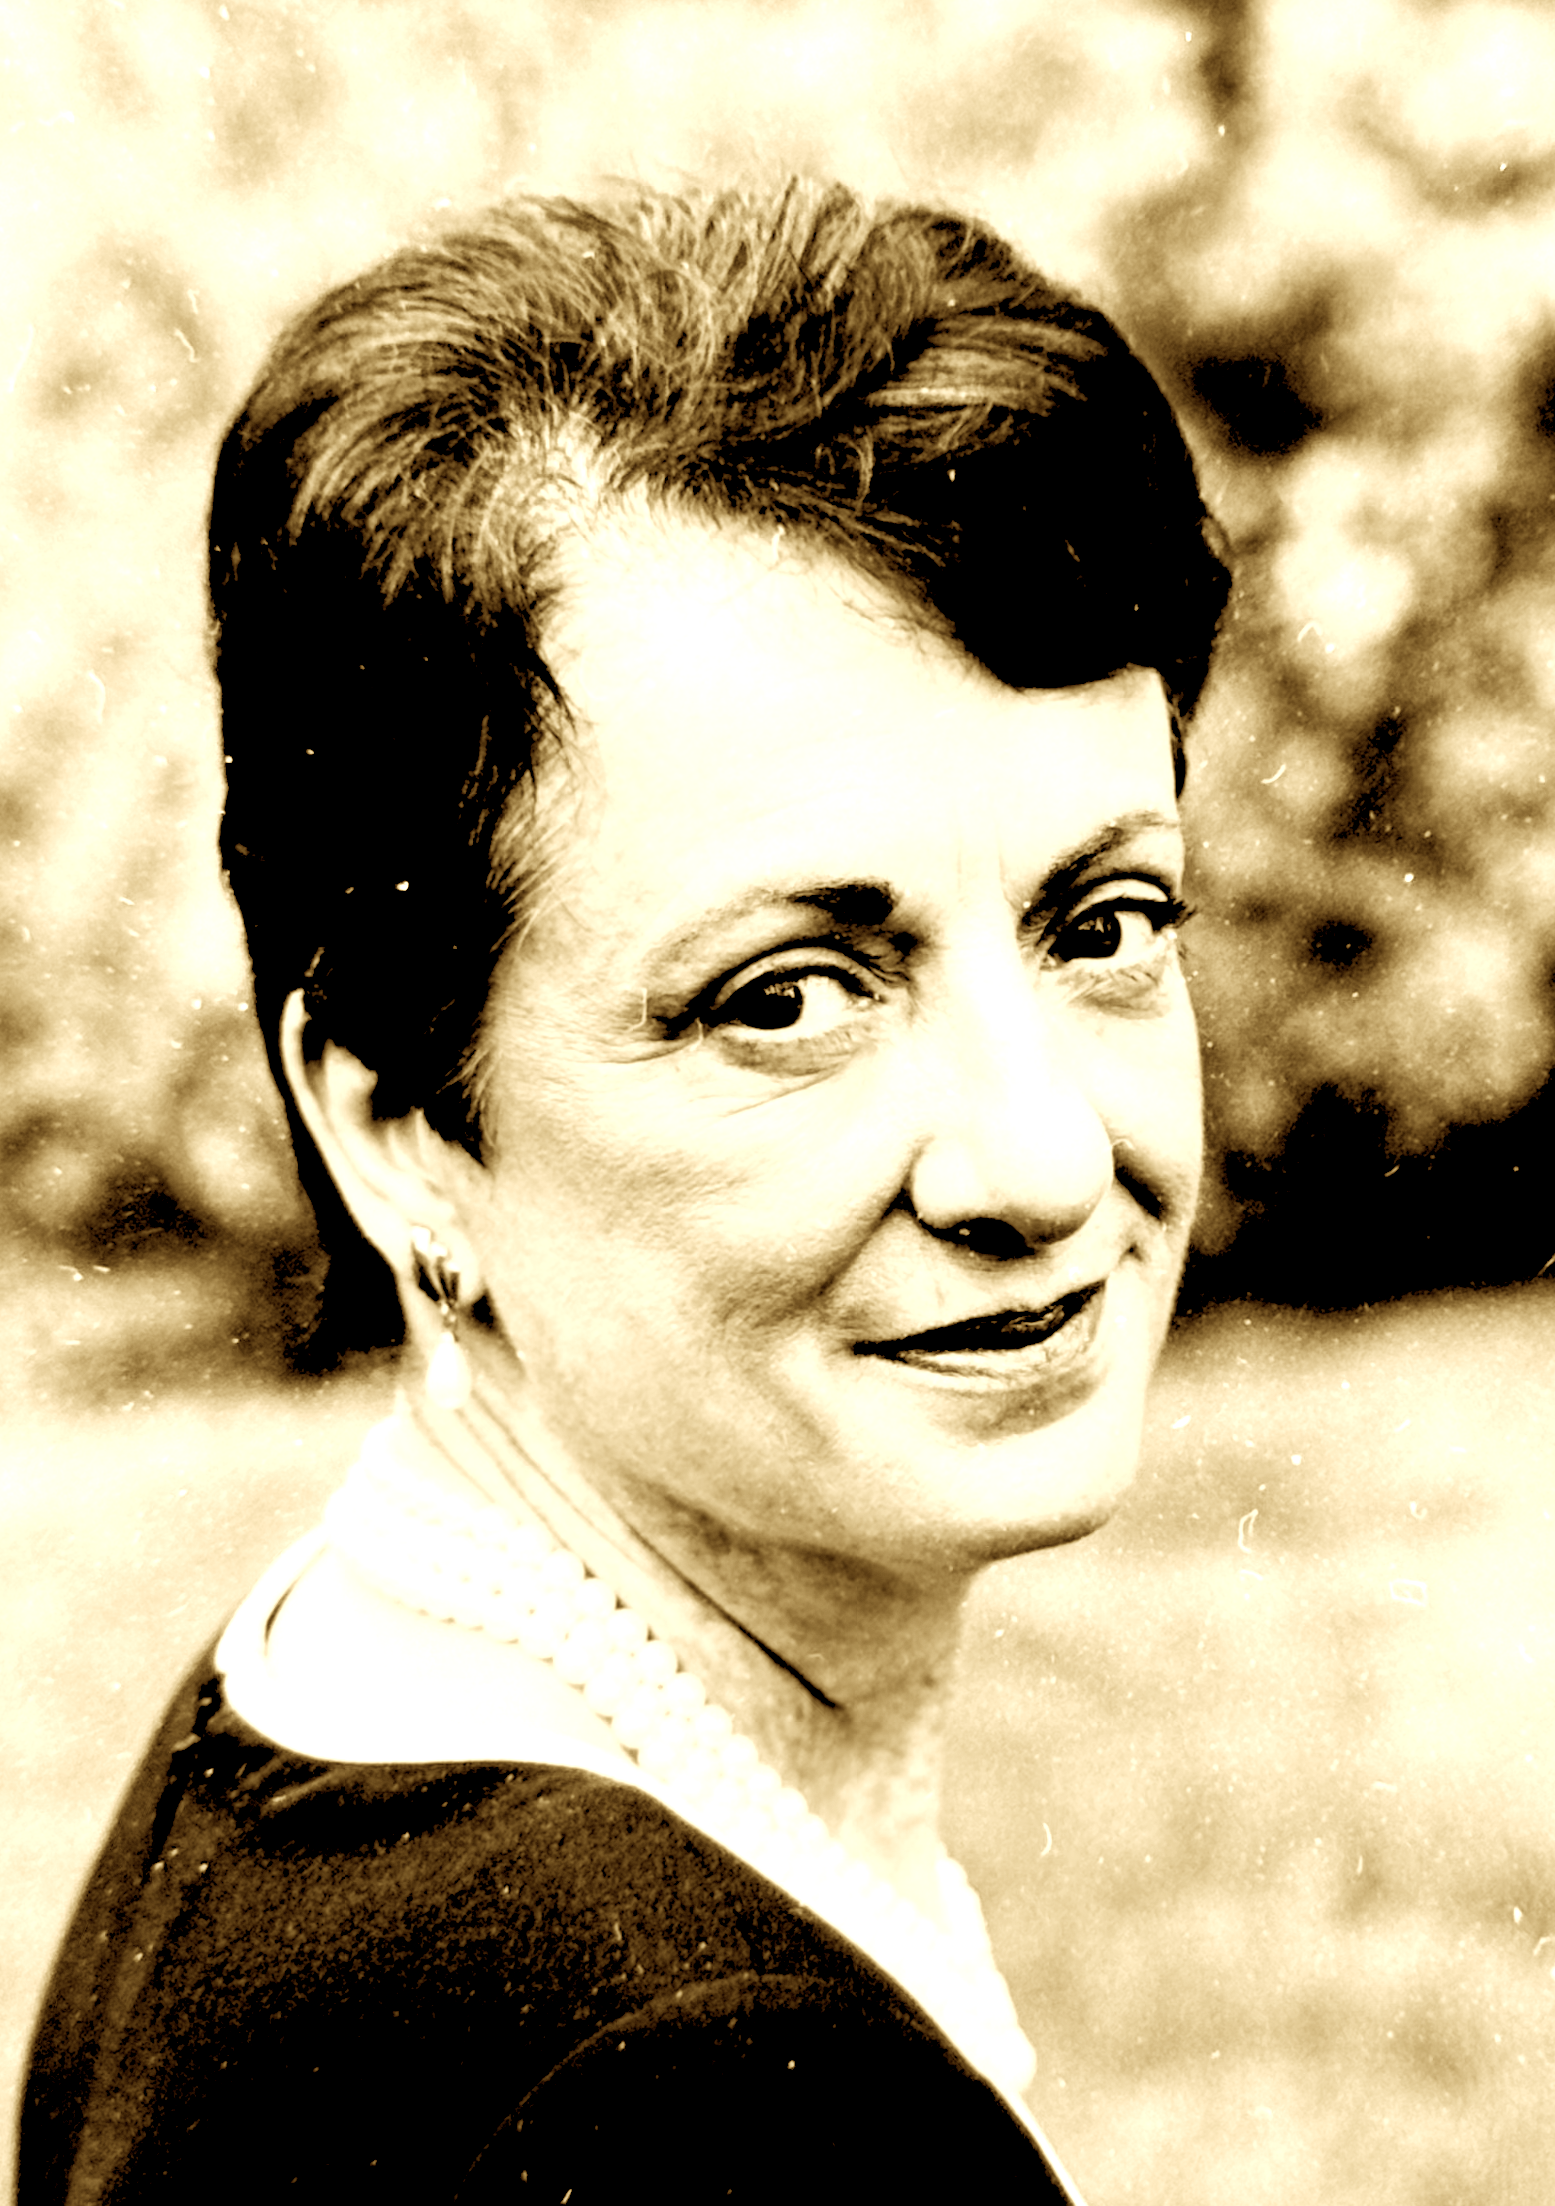
\includegraphics[width=1.75in]{img/carol-contrast.png}
    \mbox{ }\hfill\sffamily{\Large\bfseries about~the~author}
    \\[4pt]
    Carol Carpenter's poems and stories have appeared in magazines and
    journals,  \emph{Monitor}, \emph{Yankee}, 
    \emph{Redbook}, \emph{Seventeen}, \emph{Christian Science
      Monitor}, \emph{Indiana Review}, \emph{Carolina Quarterly},
    \emph{Wisconsin Review}, \emph{Quarterly West}, \emph{Snake Nation
      Review}, \emph{Birmingham Arts Journal}, \emph{Weber Journal},
    \emph{Georgetown Review}, \emph{Caveat Lector}, \emph{Orbis},
    \emph{Arabesques Review}, \emph{Fjords}, \emph{Barnwood},
    \emph{Hawai'i Review}, \emph{The Pedestal}, \emph{Soundzine}, and
    \emph{Quiddity}; in podcasts: \emph{Connecticut Review}; as anthologies:
    \emph{Poetic Voices without Borders} (Gival Press,
    2005), \emph{Tree Magic} (Sun Shine Press, 2005), \emph{Not What I
      Expected} (Paycock Press, 2007), \emph{A Walk Through my Garden}
    (Outrider Press, 2007), \emph{Wild Things} (Outrider Press, 2008)
    and \emph{Sun Dog} (Florida State University, 1997), \emph{Great
      American Poetry Show} (Muse Media, 2004), \emph{Generation to
      Generation} (Papier Mache Press, 1998), \emph{Resourceful Woman}
    (Visible Ink Press, 1994); and as chapbooks: \emph{Empress of
      Patton Avenue} (Heartsounds Press). She received 
    the Hart Crane Memorial Award, the Jean Siegel Pearson Poetry
    Award, Artists Among Us Award, and first place in the Writer's
    Digest Annual Poetry Competition (1992).  The Carol Carpenter
    Memorial Endowed Writing Scholarship is named in her honor at
    Oakland University, where she taught writing.
\end{minipage}%
\hfill\mbox{ }\hspace*{0.25in}
\end{minipage}%
%
\hspace*{-0.125in}
%
\begin{minipage}[t][9.861in][t]{0.944in}
   \vspace*{-3in}
   \hspace*{0.25in}%
    \rotatebox{270}{%
       {\fontsize{40}{40}\sffamily\bfseries poems
         $\mid$ carol carpenter}
     }
\end{minipage}%
%   
\begin{minipage}[t][9.861in][t]{6.625in}
  \noindent
  \vspace*{-2.75in} \mbox{ }
  \\
  \hspace*{1.625in} {\fontsize{86}{52}\sffamily\bfseries poems} \qquad
  \\[-4pt]
  \hspace*{1in}\rule{4.375in}{1.5pt}%  \hrule height 1pt
  \vspace*{2pt}
  \hspace*{3.115in} {\fontsize{24}{52}\sffamily carol carpenter} \qquad
  \\[5.5in]
  \hspace*{3.625in} {\sffamily\large colloquial publishing} \qquad
  \\
  \hspace*{4.585in} {\sffamily new york} \qquad
\end{minipage}
\vspace*{-8in}
\hspace*{-20in}
\end{document}


